%=========================================================================
%  RESULTADOS DEL ESTUDIO PILOTO — sección lista para manuscrito
%-------------------------------------------------------------------------
%  NOTA DE PROCEDENCIA (no aparece en el PDF compilado):
%  Todos los estadísticos de este documento provienen de la corrida completa y
%  verificada del pipeline (Experimento ALC_v5_corregido.R, v5.9, SHA-256
%  1143b36a…). Tablas de origen, relativas a «Analisis agosto v2/»:
%     · piloto/tablas/resumen_modelos_validos.csv          (ANOVA del modelo)
%     · piloto/tablas/piloto_n_palabras_calculado_EMM.csv  (medias marginales)
%     · piloto/tablas/piloto_n_palabras_calculado_contrastes_{tiempo,cond}.csv
% piloto/tablas/descriptivos_condicion_tiempo.csv (medias y DE)
% resultados/tablas/datos_completos_ancho.csv  (filtrando fuente = piloto,
% para TTR, similitud, prototipos y temas)
%  La cohorte piloto (n = 17) es una muestra INDEPENDIENTE de la principal (n = 23):
%  no es una ola del mismo estudio. No hay datos de demora y la columna n_palabras está vacía en el archivo de captura (0 de 17), de modo que la variable dependiente es el conteo n_palabras_calculado.
%  Claves de cita: se conservan las tres de tu documento (FuentesRibes2001,
%  CamachoGomez2007, Ryle2005) y se añade LopezCorral2024 con la entrada completa.
% ============================================================================

\documentclass[12pt]{article}
\usepackage[utf8]{inputenc}
\usepackage[T1]{fontenc}
\usepackage{lmodern} % fuentes vectoriales Type 1 con mapa Unicode
% rótulos de figuras y tablas en español (por defecto LaTeX usa 'Figure' y 'Table')
\renewcommand{\figurename}{Figura}
\renewcommand{\tablename}{Tabla}
\usepackage{amsmath}
\usepackage{graphicx}
\usepackage{booktabs}
\usepackage{caption}
\usepackage{subcaption}
\usepackage{geometry}
\usepackage{float}
\geometry{a4paper, margin=1in}
\usepackage{setspace}
\onehalfspacing
\graphicspath{{figuras/}} % las figuras del análisis están en esta carpeta

\title{Producción escrita y alternación de modos lingüísticos:\\ resultados del estudio piloto}
\author{}
\date{}

\begin{document}
	
	\maketitle
	
	\section{Resultados}
	
	\subsection{Participantes y muestra analítica}
	
	El estudio piloto incluyó \textbf{17 participantes}, distribuidos en tres condiciones experimentales según el modo reactivo habilitante: Texto ($n = 6$; modo leer), Audio ($n = 6$; modo escuchar) e Imagen ($n = 5$; modo observar). Cada participante produjo tres textos sucesivos sobre el mismo referente: T1, línea base sin estímulo;
	T2, tras un estímulo según la condición asignada; y T3, tras la acumulación de los tres estímulos. El diseño produjo así \textbf{51 observaciones} ($17 \times 3$).
	
	Dos rasgos de esta cohorte condicionan todas las lecturas que siguen y conviene declararlos desde el inicio. El primero es que el piloto constituye una \textbf{muestra independiente}, capturada en un momento distinto y con un instrumento distinto de los del estudio principal
	($n = 23$): no se trata de una primera ola del mismo diseño, y la columna \texttt{fuente} es lo único que permite separar ambas cohortes en los artefactos compartidos. El segundo es que la columna \texttt{n\_palabras} del archivo de captura está \textbf{vacía en la totalidad de los casos del piloto} (0 de 17), por lo que la variable dependiente empleada es el conteo verificado sobre el texto, \texttt{n\_palabras\_calculado}. Tampoco se dispone de la variable \texttt{demora}, exclusiva de la cohorte principal; en consecuencia, ningún resultado de este documento informa sobre su efecto. Esa variable sí se examina en un estudio relacionado que aún no ha sido publicado (aqui debes insertar una cita de preparacion del otro documento), por lo que sus resultados no forman parte de este documento.
	
	\subsection{Extensión del texto a través de las iteraciones}
	
	La Tabla~\ref{tab:desc_piloto} presenta los estadísticos descriptivos de la extensión por condición y momento del episodio.
	
	\begin{table}[H]
		\centering
		\caption{Extensión del texto (\texttt{n\_palabras\_calculado}): media (desviación estándar) y mediana por condición y momento. Estudio piloto, $n = 17$.}
		\label{tab:desc_piloto}
		\begin{tabular}{l c c c c}
			\toprule
			Condición & Momento & $n$ & $M$ ($DE$) & Mediana \\
			\midrule
			Texto  & T1 & 6 & 143.67 (53.40) & 140.00 \\
			Texto  & T2 & 6 & 116.83 (60.65) &  95.50 \\
			Texto  & T3 & 6 & 116.50 (65.81) & 110.50 \\
			\midrule
			Audio  & T1 & 6 & 133.67 (62.04) & 116.50 \\
			Audio  & T2 & 6 & 172.17 (60.02) & 160.50 \\
			Audio  & T3 & 6 & 216.83 (114.97) & 171.00 \\
			\midrule
			Imagen & T1 & 5 &  97.80 (77.35) &  90.00 \\
			Imagen & T2 & 5 & 103.20 (80.35) &  80.00 \\
			Imagen & T3 & 5 & 110.60 (47.28) &  86.00 \\
			\bottomrule
		\end{tabular}
		\par\smallskip
		\noindent\begin{minipage}{\textwidth}
			\footnotesize
			\emph{Nota}: las desviaciones estándar son del mismo orden que las medias en casi todas las celdas, con la condición Imagen en T1 como caso extremo. La mediana se incluye porque las distribuciones son asimétricas.
		\end{minipage}
	\end{table}
	
	\vspace{0.5\baselineskip} % opcional: reduce el espacio entre tablas
	
	Se ajustó un modelo lineal mixto con efectos fijos de \texttt{condicion}, \texttt{tiempo} y su interacción, e intercepto aleatorio por participante (estimación REML, grados de libertad Satterthwaite). La Tabla~\ref{tab:anova_piloto} resume la prueba de efectos fijos.
	
	\begin{table}[H]
		\centering
		\caption{ANOVA de tipo III (Satterthwaite) del modelo mixto para \texttt{n\_palabras\_calculado}. Estudio piloto, 51 observaciones de 17 participantes.}
		\label{tab:anova_piloto}
		\begin{tabular}{l c c c c}
			\toprule
			Efecto & $F$ & gl num. & gl den. & $p$ \\
			\midrule
			Condición                & 1.701 & 2 & 14 & .218 \\
			Tiempo                   & 1.845 & 2 & 28 & .177 \\
			Condición $\times$ tiempo & \textbf{3.642} & 4 & 28 & \textbf{.016} \\
			\bottomrule
		\end{tabular}
		\par\smallskip
		\noindent\begin{minipage}{\textwidth}
			\footnotesize
			\emph{Nota}: $R^2$ marginal $= .208$; $R^2$ condicional $= .800$. La interacción es el único efecto que alcanza el umbral convencional.
		\end{minipage}
	\end{table}
	
	El modelo explicó el \textbf{20.8\%} de la varianza atribuible a los efectos fijos ($R^2$ marginal) y el \textbf{80.0\%} de la varianza total al incorporar el intercepto aleatorio ($R^2$ condicional). Dicho de otro modo, cuatro quintas partes de la variación que esta presente en la extensión de los textos se deben a diferencias \emph{entre} participantes, y no a la condición ni al momento del episodio.

	En este estudio piloto \textbf{no se encuentra un efecto principal de tiempo}, es decir, la extensión no aumenta de manera general con la repetición ($F(2,28) = 1.845$, $p = .177$). Lo que sí esta presente y emerge es una \textbf{interacción condición $\times$ tiempo} ($F(4,28) = 3.642$, $p = .016$), donde la trayectoria de la extensión depende del modo reactivo por el que se estableció el contacto con el referente. De la misma manera podemos determinar que las medias marginales estimadas (Tabla~\ref{tab:emm_piloto}) muestran que ese efecto procede de una sola condición.
	
	\begin{table}[H]
		\centering
		\small
		\setlength{\tabcolsep}{4pt}
		\caption{Medias marginales estimadas (EM), error estándar (SE) e intervalo de confianza del 95\% de la extensión, por condición y momento. Estudio piloto.}
		\label{tab:emm_piloto}
		\begin{tabular}{@{}l c c c c c@{}}
			\toprule
			Condición & Momento & EM & SE & IC 95\% inf. & IC 95\% sup. \\
			\midrule
			Texto  & T1 & 143.67 & 29.30 &  82.52 & 204.82 \\
			Texto  & T2 & 116.83 & 29.30 &  55.68 & 178.00 \\
			Texto  & T3 & 116.50 & 29.30 &  55.35 & 177.65 \\
			\midrule
			Audio  & T1 & 133.67 & 29.30 &  72.52 & 194.82 \\
			Audio  & T2 & 172.17 & 29.30 & 111.02 & 233.32 \\
			Audio  & T3 & 216.83 & 29.30 & 155.68 & 278.00 \\
			\midrule
			Imagen & T1 &  97.80 & 32.10 &  30.81 & 164.79 \\
			Imagen & T2 & 103.20 & 32.10 &  36.21 & 170.19 \\
			Imagen & T3 & 110.60 & 32.10 &  43.61 & 177.59 \\
			\bottomrule
		\end{tabular}
		\par\smallskip
		\noindent\begin{minipage}{\textwidth}
			\footnotesize
			\emph{Nota}: estimaciones obtenidas con \texttt{emmeans} sobre el modelo ajustado con \texttt{lmerTest} (gl $\approx 19.85$). Los intervalos son amplios: con 5 o 6 participantes por condición, el modelo no permite estimaciones precisas.
		\end{minipage}
	\end{table}
	
	Los contrastes \emph{a posteriori} con ajuste de Holm permiten precisar el patrón. \textbf{Entre momentos dentro de cada condición}, donde se presenta Audio mostró un aumento significativo de T1 a T3 ($\Delta = -83.17$ palabras, $p = .001$), con sus dos pasos parciales, es decir, de T1 a T2 y de T2 a T3 con valores de $p$ próximos al umbral convencional de significación ($\Delta = -38.50$ y $-44.67$, respectivamente, ambos $p = .082$). En las condiciones donde se presenta tanto el Texto, como la Imagen ningún contraste alcanzó significación (Texto: T1--T2 $p = .610$, T1--T3 $p = .610$, T2--T3 $p = .987$; Imagen: los tres $p = 1.000$); de hecho, en Texto la tendencia fue de \emph{disminución} de T1 a T2 y a T3. \textbf{Entre condiciones en cada momento}, no se observaron diferencias significativas: en T1 y T2 todos los contrastes resultaron claramente no significativos ($p$ entre .385 y .912); en T3, las comparaciones Audio--Texto ($\Delta = 106.23$) y Audio--Imagen ($\Delta = 106.23$) se quedaron en $p = .072$, por debajo del umbral pero sin alcanzarlo.
	
	Lo observado en este estudio piloto revela que la extensión del texto evoluciona de forma \textbf{heterogénea según el modo reactivo y no de manera uniforme}: la condición de Audio es la única que refleja un crecimiento sostenido en los tres momentos, frente a un modo Texto que se estanca o retrocede y una Imagen que se mantiene plana. Puesto que la diferencia entre Audio y Texto en T3 no alcanza significación y las muestras son pequeñas (5--6 participantes por grupo), este comportamiento debe interpretarse de forma \textbf{exploratoria}: sugiere una dirección, pero sin establecer diferencias definitivas.
	
	Las Figuras~\ref{fig:piloto_trayectoria} a \ref{fig:piloto_distribucion} presentan este patrón a partir de las trayectorias estimadas, las trayectorias individuales y la distribución por condición y momento. Asimismo, la Figura~\ref{fig:piloto_diagnosticos} documenta el diagnóstico del modelo. Todas estas gráficas se generaron en la corrida del pipeline y emplean \texttt{n\_palabras\_calculado}, la variable dependiente de esta cohorte.
	
	La Figura~\ref{fig:piloto_trayectoria} muestra las trayectorias de la extensión por condición. Cada línea representa la media marginal estimada por el modelo mixto, con su intervalo de confianza del 95\%. Las tres condiciones parten de niveles distintos, y solo Audio asciende de forma sostenida (de 133.67 a 216.83 palabras); Texto desciende entre T1 y T2 y se mantiene después; Imagen permanece prácticamente plana (de 97.80 a 110.60). La divergencia entre las tres líneas es la representación de la interacción condición $\times$ tiempo ($F(4,28) = 3.642$, $p = .016$), único efecto significativo del modelo. La amplitud de las bandas refleja la base de 5 o 6 participantes por condición, y es la razón por la que el patrón se reporta como exploratorio.
	
	\vspace{0.2cm}
	
	\begin{figure}[H]
		\centering
		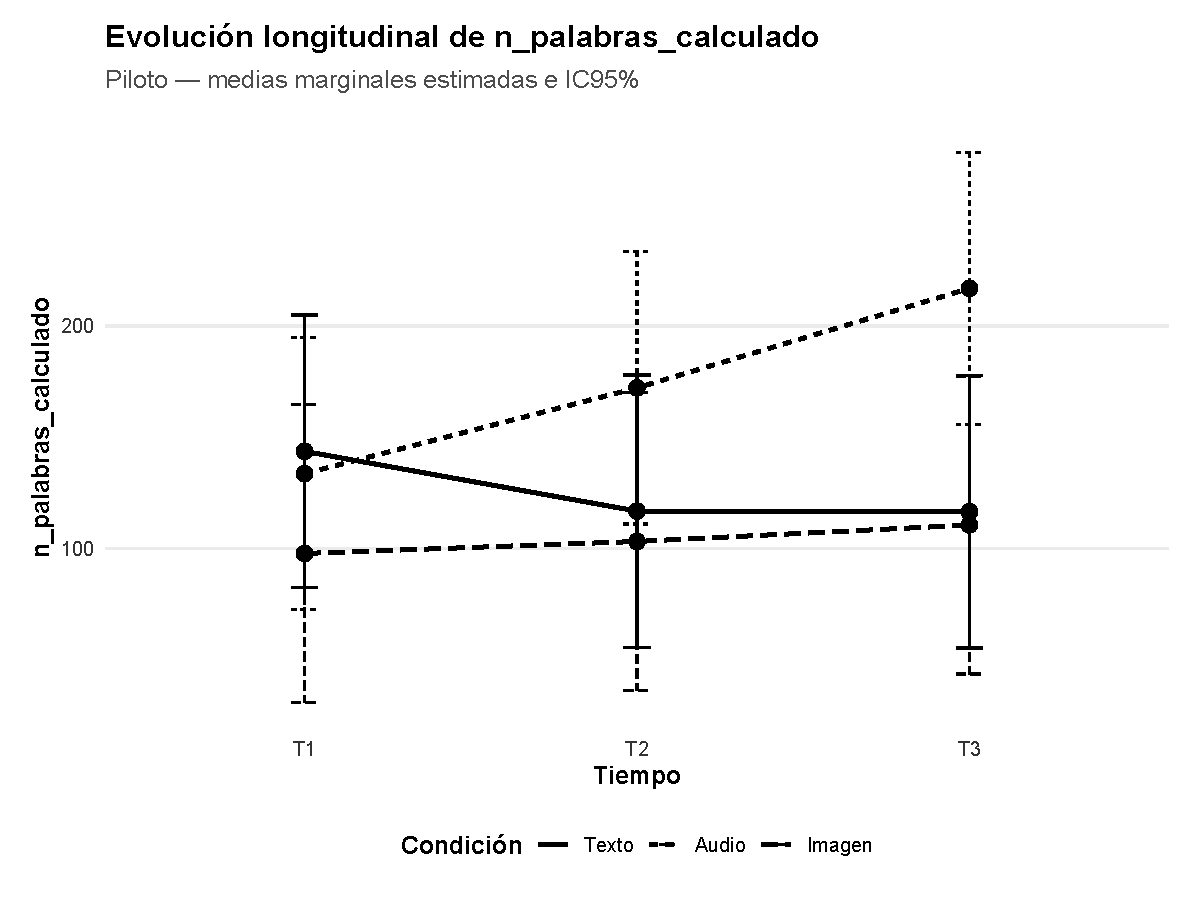
\includegraphics[width=0.92\textwidth]{PILOTO_n_palabras_calculado_ES_trayectoria.pdf}
		\caption{Trayectorias de la extensión por condición.}
		\label{fig:piloto_trayectoria}
	\end{figure}
	
	\vspace{0.2cm}
	
	La Figura~\ref{fig:piloto_individuales} presenta las trayectorias individuales de la extensión para cada participante superpuestas a la tendencia grupal de su respectiva condición. Esta visualización ilustra la fuerte heterogeneidad que explica la diferencia entre la varianza explicada marginal ($R^2 = .208$) y la condicional ($R^2 = .800$), dado que múltiples trayectorias se cruzan y muestran a participantes que triplican su punto de partida mientras que otros lo reducen. De este modo, la gráfica advierte claramente que las medias reportadas en la Figura~\ref{fig:piloto_trayectoria} no deben interpretarse como el comportamiento de un escritor típico.
	
	\vspace{0.2cm}
	
	\begin{figure}[H]
		\centering
		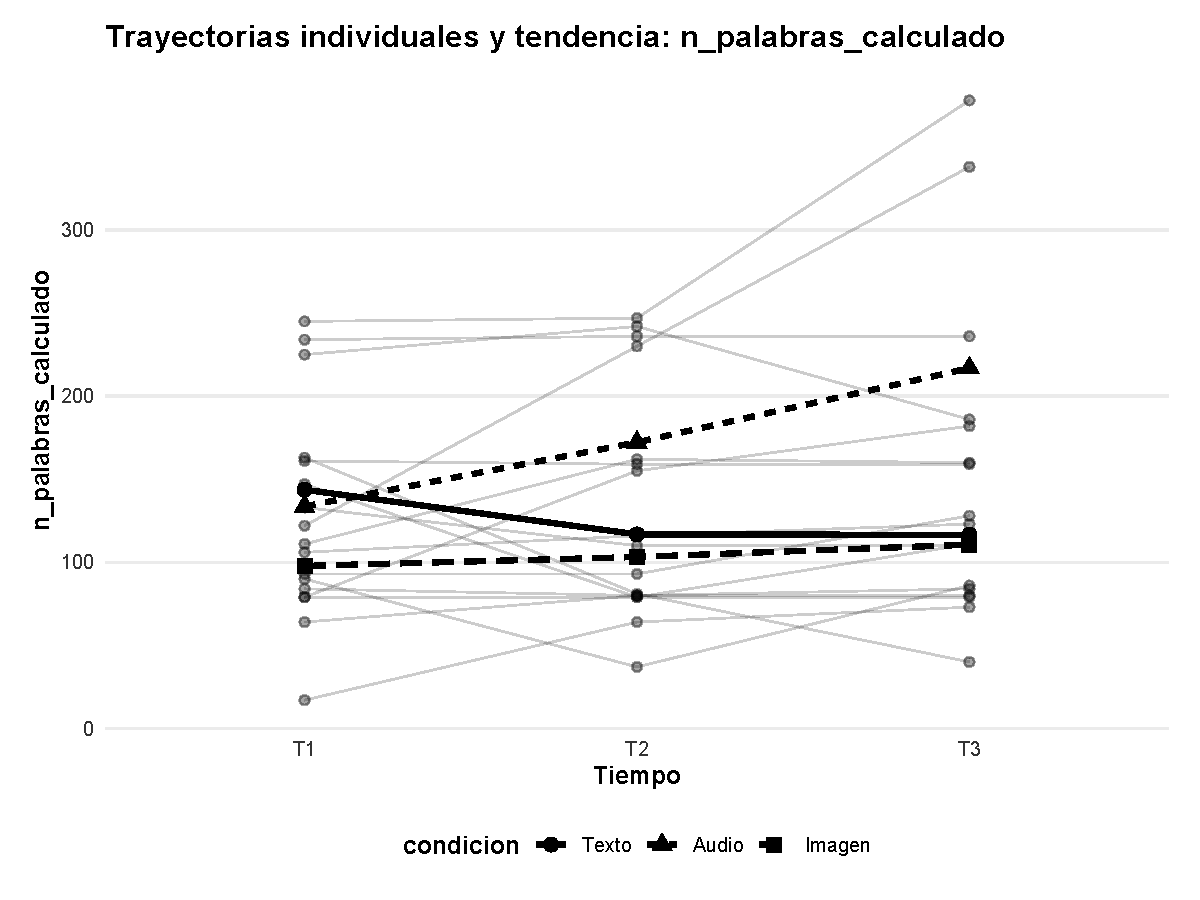
\includegraphics[width=0.92\textwidth]{PILOTO_n_palabras_calculado_ES_individuales.pdf}
		\caption{Trayectorias individuales de la extensión por participante.}
		\label{fig:piloto_individuales}
	\end{figure}
	
	\vspace{0.2cm}
	
	La Figura~\ref{fig:piloto_distribucion} muestra la distribución de la extensión por condición y momento mediante diagramas de caja que integran las observaciones individuales superpuestas. En esta representación destaca que el grupo de Audio en T3 presenta la mayor dispersión ($DE = 114.97$, frente a un rango de $47$ a $81$ en el resto de las celdas) e incluye el texto más extenso del piloto con 378 palabras, en claro contraste con la condición de Imagen, cuyas distribuciones resultan mucho más compactas. Precisamente esta dispersión es la que sostiene el contraste entre T1 y T3 para la condición Audio ($\Delta = -83.17$, $p = .001$) y, al mismo tiempo, explica por qué dicho efecto depende de un número reducido de casos.
	
	\vspace{0.2cm}
	
	\begin{figure}[H]
		\centering
		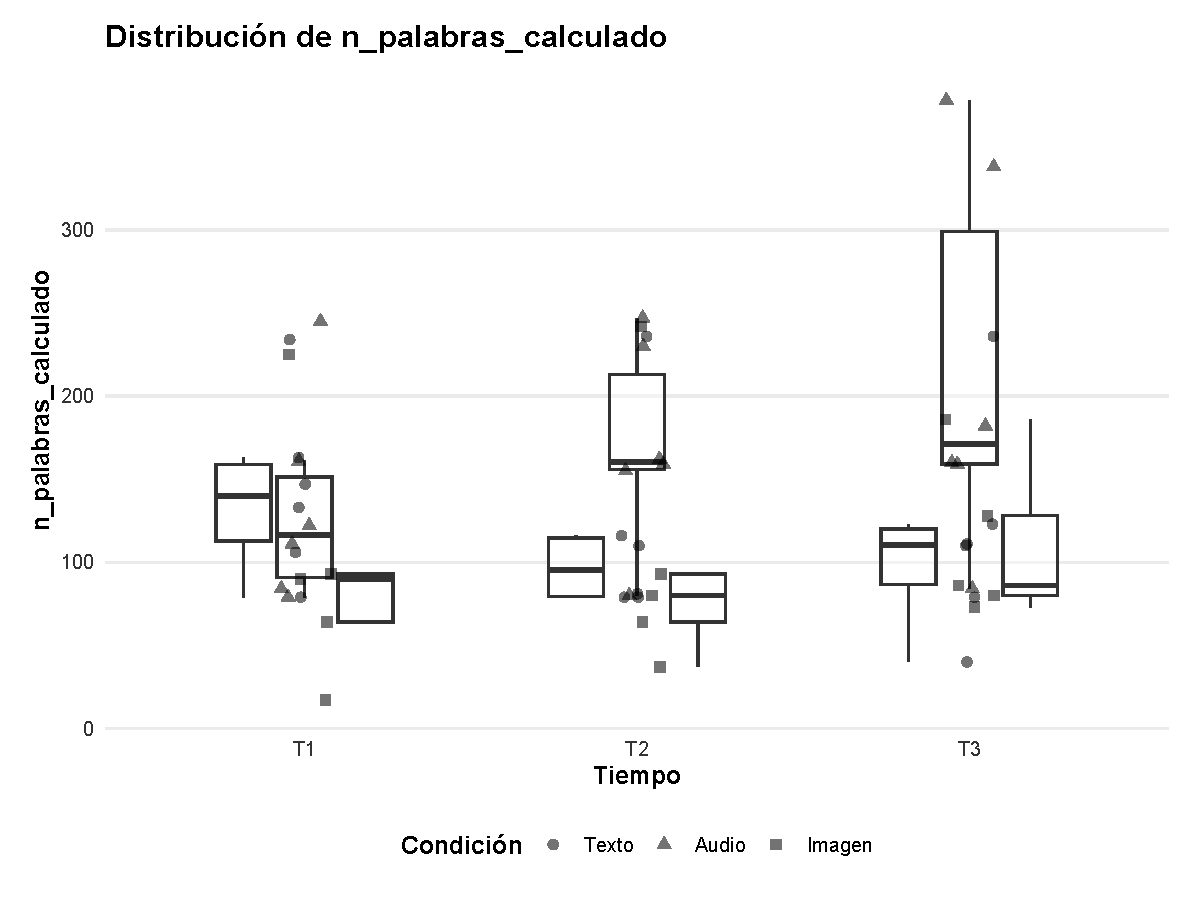
\includegraphics[width=0.92\textwidth]{PILOTO_n_palabras_calculado_ES_distribucion.pdf}
		\caption{Distribución de la extensión por condición y momento.}
		\label{fig:piloto_distribucion}
	\end{figure}
	
	\vspace{0.2cm}
	
	La Figura~\ref{fig:piloto_diagnosticos} documenta el diagnóstico del modelo mixto generado con el paquete \texttt{performance}, el cual evalúa parámetros como la linealidad de los residuos frente a los valores ajustados, la homogeneidad de la varianza, la normalidad de los residuos, la colinealidad y la presencia de observaciones influyentes. Los resultados indican que en esta cohorte no se aprecian violaciones relevantes a dichos supuestos, ya que la prueba de Shapiro-Wilk sobre los residuos arroja un valor de $W = 0.9915$ ($p = .974$) y los residuos escalados se mantienen en un rango de $-1.71$ a $1.97$. En consecuencia, ninguna de las 51 observaciones supera el umbral de $|2.5|$ que emplea el pipeline para identificar casos influyentes, lo que permitió que el modelo convergiera sin problemas de singularidad. Este comportamiento resulta especialmente instructivo al contrastarlo con el análisis del conjunto completo, puesto que allí ese mismo criterio marcó 115 de 120 observaciones e impidió estimar el reajuste, mientras que en este piloto no hubo ningún caso que requiriera exclusión.
	
	\begin{figure}[H]
		\centering
		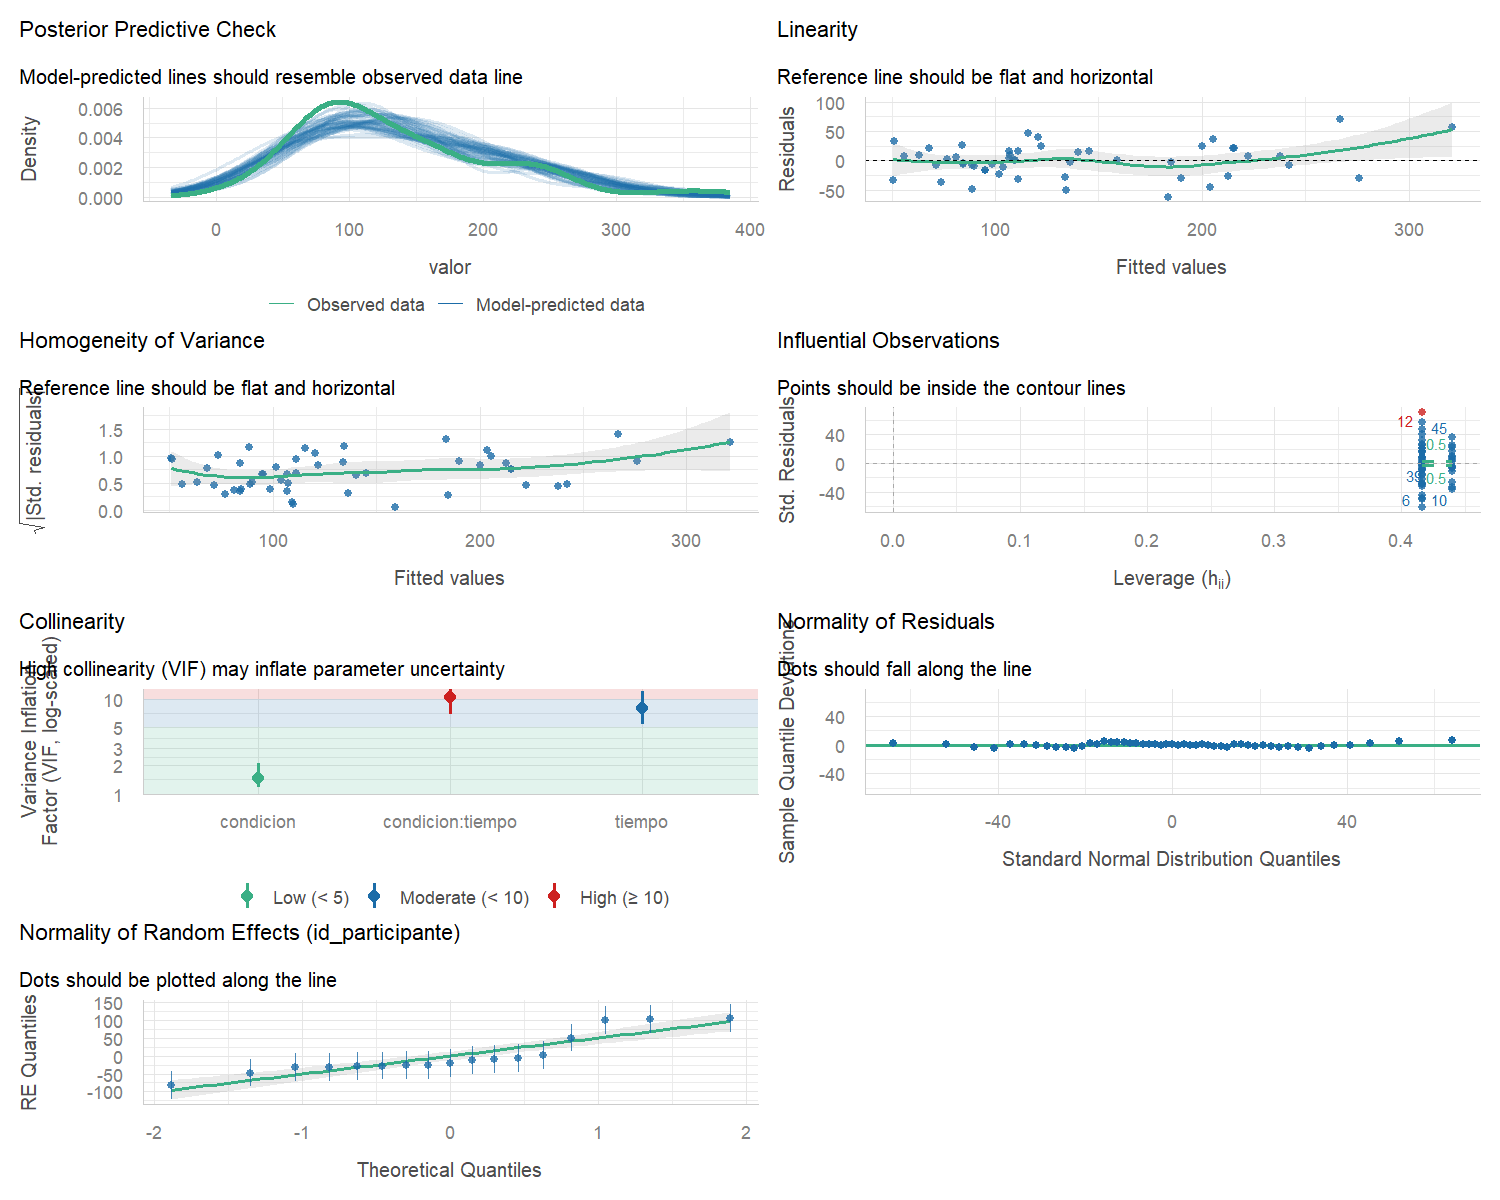
\includegraphics[width=0.92\textwidth]{piloto_n_palabras_calculado_check_model.png}
		\caption{Diagnóstico del modelo mixto.}
		\label{fig:piloto_diagnosticos}
	\end{figure}
	
	\subsection{Diversidad léxica}
	
	El Type-Token Ratio (TTR) del piloto partió de una media de $0.822$ con una desviación estándar de $0.090$ en T1, pasando a $0.848$ con una dispersión de $0.084$ en T2, para finalmente situarse en $0.846$ con una desviación de $0.092$ en T3. Al ajustar un modelo mixto con la misma especificación que el anterior, los resultados no arrojaron un efecto principal de la condición al presentar un valor $F(2,14)$ de $0.057$ ($p = .944$), ni tampoco un efecto del tiempo tras arrojar una $F(2,28)$ de $2.079$ ($p = .144$). Sin embargo, el análisis confirmó una interacción significativa entre condición y tiempo evidenciada por una $F(4,28)$ de $2.830$ con una $p$ de $.043$, donde el modelo alcanzó una varianza explicada marginal de $.065$ y una condicional de $.805$.
	
	Resulta conveniente distinguir dos lecturas de estos hallazgos. En primer lugar, la diversidad léxica del piloto \textbf{no disminuyó} a lo largo del episodio, puesto que los textos de T2 y T3 no resultaron ser léxicamente más pobres que los de T1. A esto se suma que la varianza marginal del modelo es prácticamente nula, lo que indica que la condición y el momento de evaluación explican una porción mínima del comportamiento del TTR. En segundo lugar, la interacción encontrada reproduce la misma tendencia observada previamente en la extensión, donde una condición específica se comporta de manera distinta a las otras dos. Este patrón resulta coherente si se considera que ambas medidas responden al mismo contraste, aunque también funciona como una advertencia de que el TTR no opera con independencia de la condición analizada. Finalmente, es fundamental recordar que este índice está supeditado a la longitud total del texto, por lo que cualquier comparación entre momentos que presenten extensiones distintas exige una estricta cautela interpretativa.
	
	\subsection{Estabilidad semántica entre segmentos}
	
	La similitud coseno entre los vectores de los tres textos de cada participante, calculada mediante el modelo \texttt{paraphrase-multilingual-MiniLM-L12-v2}, resultó ser mayor entre los momentos T2 y T3 al alcanzar una media de $0.937$ con una desviación estándar de $0.100$. Esta cifra supera la similitud observada entre T1 y T2, que registró una media de $0.843$ y una dispersión de $0.198$, así como la calculada entre T1 y T3, cuya media fue de $0.802$ con una desviación de $0.204$. Al evaluar estos datos a través de un modelo mixto que incluyó el par de comparación como único efecto fijo y un intercepto aleatorio por participante, se confirmó un efecto significativo del par evidenciado por una $F(2,32)$ de $5.409$ con una $p$ de $.0095$.
	
	Este ordenamiento refleja el comportamiento esperado si el episodio avanzara mediante aproximaciones sucesivas a un mismo referente previamente escrito. En este sentido, el cambio más pronunciado ocurre entre el primer texto, redactado sin contacto previo con el estímulo, y el segundo, mientras que la variación menor se da entre el segundo y el tercero. No obstante, los valores absolutos deben interpretarse con reserva debido a que la similitud media entre T1 y T2 incluye casos con registros tan bajos como $0.34$. En definitiva, es precisamente esta acusada variabilidad individual, por encima de la tendencia central, la que explica que el efecto del par resulte moderado.
	
	\subsection{Contenido temático y prototipos (análisis exploratorio)}
	
	Con el propósito de profundizar en la dimensión semántica de las narrativas, se aplicaron diez diccionarios temáticos construidos específicamente alrededor de los ejes visuales y afectivos que caracterizan la estética de Hopper. Para asegurar la comparabilidad entre textos de distinta longitud, la frecuencia de aparición de estos conceptos se estandarizó y se expresa como una tasa por cada 1000 palabras. La Tabla~\ref{tab:temas_piloto} detalla la evolución de estas tasas a lo largo de los tres momentos de evaluación, ofreciendo una panorámica descriptiva de cómo fluctúan los focos de atención de los participantes durante el episodio. A la par de este escrutinio temático, se calcularon los cambios de proximidad hacia diversos prototipos semánticos tomando como referencia el contraste entre el texto inicial y el final.
	
	\begin{table}[H]
		\centering
		\caption{Tasas por 1000 palabras de los diccionarios temáticos, por momento del episodio. Estudio piloto ($n = 17$).}
		\label{tab:temas_piloto}
		\begin{tabular}{l c c c}
			\toprule
			Tema & T1 & T2 & T3 \\
			\midrule
			Soledad              & 28.98 & 27.95 & 27.20 \\
			Espacio              & 26.66 & 22.05 & 22.04 \\
			Objetos              & 21.31 & 20.39 & 25.66 \\
			Emociones negativas  &  2.56 &  5.90 &  5.04 \\
			Luz y sombra         &  4.03 &  1.66 &  1.17 \\
			Pasividad            &  4.02 &  2.19 &  3.30 \\
			Duda                 &  1.62 &  2.32 &  2.85 \\
			Espera               &  1.54 &  0.98 &  1.26 \\
			Incomunicación       &  0.00 &  0.51 &  0.48 \\
			Desconexión          &  0.00 &  0.00 &  0.00 \\
			\bottomrule
		\end{tabular}
	\end{table}
	
	Al analizar las métricas subyacentes a la tabla, cabe destacar que las desviaciones estándar omitidas por cuestiones de brevedad resultan del mismo orden o incluso mayores que las medias en prácticamente todos los renglones, lo cual refleja una alta heterogeneidad entre los participantes. Asimismo, resalta que dos temas del diccionario relativos a la incomunicación y la desconexión prácticamente no figuran en el corpus del piloto. De hecho, en el caso de la desconexión la tasa es exactamente cero en los tres momentos, lo que indica de manera tajante que los términos elegidos para operacionalizar dicho constructo no lograron representación alguna en estos textos.
	
	Por su parte, los cambios de proximidad a los prototipos semánticos entre el primer y el tercer momento resultaron pequeños en todos los casos. Las variaciones más pronunciadas correspondieron a la tristeza con un incremento de $0.048$ y una desviación estándar de $0.082$, seguidas por las emociones negativas con un aumento de $0.045$ y una dispersión de $0.092$, así como por la ansiedad y el malestar, cuyo avance fue de $0.035$ con una desviación de $0.090$. El resto de los constructos analizados se mantuvo por debajo de una magnitud absoluta de $0.021$. En la totalidad de estos casos la desviación estándar supera ampliamente a la media y la mediana presenta un valor inferior, lo cual constituye un fuerte indicio de que el cambio se concentra en un número reducido de participantes y descarta la existencia de un desplazamiento sistemático a nivel grupal. Resulta importante subrayar que estos análisis no fueron sometidos a corrección por comparaciones múltiples pese a involucrar 20 constructos y 10 temas, ni se les aplicó ninguna prueba inferencial, motivo por el cual sus hallazgos se reportan con un carácter estrictamente exploratorio y descriptivo.
	
	Finalmente, y a modo de referencia puramente descriptiva que carece de valor inferencial a causa del tamaño reducido de los grupos, se calculó la distancia euclidiana entre T1 y T3 dentro del espacio reducido por componentes principales. En la condición de Audio esta métrica alcanzó una media de $2.30$ con una desviación de $2.87$, mientras que en Texto se ubicó en $5.21$ con una dispersión de $4.22$, para luego ascender en la condición de Imagen hasta una media de $8.26$ con una desviación de $3.81$. Al interpretar estas cifras debe tenerse presente que dicho espacio dimensional se ajustó tomando como base los 120 vectores correspondientes al conjunto completo de datos del piloto y el estudio principal, por lo que las distancias aquí reportadas no son independientes de esa solución algorítmica global.
	
	\section{Discusión}
	
	\subsection{Síntesis del patrón}
	
	El piloto ofrece un patrón que resulta ser el inverso del documentado en la cohorte principal, por lo que conviene enunciarlo con precisión antes de proceder a su interpretación. En este caso, la extensión del texto \textbf{no} aumenta de manera general con la repetición al presentar un valor $F(2,28)$ de $1.845$ ($p = .177$), sino que depende fuertemente del modo reactivo asignado. Esto queda evidenciado por una interacción significativa con una $F(4,28)$ de $3.642$ ($p = .016$), la cual se explica porque la condición de Audio experimenta un crecimiento claro de $83.17$ palabras entre el primer y el tercer momento ($p = .001$), mientras que la modalidad de Texto se mantiene o retrocede y la de Imagen permanece plana. Paralelamente, la diversidad léxica no decae a lo largo del ejercicio y la similitud semántica logra estabilizarse desde el segundo paso del episodio. En cuanto a los cambios de contenido temático y de proximidad a los prototipos, estos resultan pequeños y marcados por la heterogeneidad. Como colofón a este patrón, cabe señalar que aproximadamente cuatro quintas partes de la varianza en la extensión corresponden a diferencias individuales entre los participantes, alcanzando una varianza condicional explicada de $.800$.
	
	\subsection{Habilitación lingüística: ¿contacto con el referente o modo específico?}
	
	Para interpretar este patrón, la distinción teórica más productiva proviene de la literatura revisada en el propio artículo. En dicho marco, la habilitación lingüística se define operativamente como la facilitación de un desempeño en un modo activo generada a partir de la exposición a un modo reactivo (Camacho \& Gómez, 2007; Gómez, 2005; Tamayo et al., 2010, citados en López Corral et al., 2024), lo cual remite a la manera en que el acto de leer, escuchar u observar termina por afectar la escritura. Bajo esta lógica, si la facilitación fuera un simple efecto general derivado de ``tener algo que decir'', bastaría con el mero contacto con el referente sin importar su modalidad. Por el contrario, si esta facilitación estuviera ligada a un modo específico, cada condición experimental debería producir un efecto claramente distinguible.
	
	El artículo de referencia es explícito al advertir que este debate aún no está resuelto y que la evidencia disponible apunta a un fenómeno mucho más amplio que la simple dupla complementaria. Específicamente, señala que la habilitación lingüística de la escritura también se ha documentado en relación con los modos de \textbf{escuchar} y \textbf{observar}, los cuales \emph{no} forman un par natural con la producción escrita. De esto se concluye que la interrelación funcional de la escritura parece trascender a la lectura para abarcar otras modalidades perceptuales (López et al., 2019, 2020, citados en López Corral et al., 2024). En este contexto, el patrón observado en el piloto, donde la única condición que logra extender el texto es precisamente la auditiva, concuerda perfectamente con lo que dicha evidencia empírica anticiparía, alejándose de lo que predeciría una interpretación estricta centrada de forma exclusiva en el binomio de escribir y leer.
	
	A pesar de esta coherencia teórica, existen tres razones fundamentales que impiden elevar este comportamiento a la categoría de hallazgo concluyente. La primera de ellas radica en que los contrastes directos entre las condiciones al llegar al tercer momento arrojaron una $p$ de $.072$ tanto al comparar Audio contra Texto como frente a Imagen, por lo que la diferencia medular del argumento no logró alcanzar el umbral de significación estadística. La segunda razón obedece a que este efecto se sostiene sobre una muestra de apenas seis participantes, una base tan reducida que permitiría a una única trayectoria atípica generar toda la interacción observada. Finalmente, el tercer y más importante motivo es que este patrón no logra replicarse en la cohorte principal. En dicha muestra, la interacción resulta prácticamente nula al presentar una $F(4,40)$ de $0.075$ ($p = .989$), consolidando el tiempo general como el efecto dominante. Esta discrepancia metodológica se corrobora mediante una comparación formal entre ambas cohortes que evalúa la interacción de la fuente de los datos por el tiempo evaluado. Dicho análisis arrojó una $F(2,68)$ de $6.848$ con una $p$ de $.002$, lo cual confirma que las trayectorias de crecimiento difieren de manera significativa entre el piloto y el estudio principal, aun cuando el nivel general de extensión escrita entre ambos grupos no presente variaciones destacables ($p = .939$).
	
	En consecuencia, la lectura metodológicamente defendible de estos resultados debe orientarse hacia la \textbf{generación de hipótesis}. El estudio piloto logra formular la conjetura de una habilitación lingüística impulsada específicamente por el modo de escuchar, pero carece de la robustez necesaria para aportar evidencia definitiva al respecto. El valor real de este hallazgo reside en que dicha hipótesis resulta empíricamente formulable, medible y falsable, y encuentra su primer límite en la cohorte principal, la cual no logra confirmarla al exhibir en cambio un efecto generalizado del tiempo. Por consiguiente, cualquier diseño experimental futuro que pretenda someter a prueba esta dinámica requerirá de una asignación balanceada, un tamaño de muestra por condición lo suficientemente amplio como para sostener el análisis de interacción, y la precaución insoslayable de declarar el contraste entre Audio y Texto como el objetivo principal del estudio desde antes de iniciar la recolección de los datos.
	
	\subsection{Segmentación del episodio y extensión del mismo}
	
	El marco teórico de este estudio propone entender el episodio de escritura como una actividad extensible y segmentable. Bajo este modelo, un primer corte, denominado Segmento A, corresponde al contacto con el referente y a la subsecuente producción de un texto. A este le sigue un segundo corte, o Segmento B, centrado en la interacción con el referente original o con su versión escrita con la finalidad de modificarla, lo cual da origen a lo que López Corral y colaboradores (2024) conceptualizan como el \emph{Referente AB}. El diseño metodológico del piloto implementa precisamente esta segmentación a través de dos cortes temporales que transicionan desde T1 hacia T2, y posteriormente de T2 hacia T3.
	
	Al evaluar los contrastes de la condición de Audio es posible describir este fenómeno con gran precisión. El cambio acumulado entre el primer y el tercer momento resulta estadísticamente significativo con una $p$ de $.001$, mientras que ninguno de los dos pasos parciales logra alcanzar dicho umbral por separado al registrar ambos una $p$ de $.082$. Por lo tanto, no se está ante un salto abrupto asociado al primer contacto con el estímulo, sino ante un crecimiento \textbf{gradual a lo largo de los dos segmentos} que únicamente se vuelve detectable al sumarse. En contraste, dentro de la condición de Texto el segundo segmento no añade volumen respecto al primero ($p = .987$), marcando incluso una tendencia descriptiva de retorno al nivel inicial. Así, la segmentación del episodio se refleja de manera marcadamente desigual según el modo reactivo asignado, permitiendo que en la condición auditiva la actividad se extienda a lo largo de sus segmentos, dinámica que no logra cristalizarse en la modalidad de lectura.
	
	Llegado a este punto resulta indispensable subrayar una limitación conceptual en esta operacionalización. Mientras que la teoría habla de la extensión \emph{del episodio} para referirse a una actividad que se prolonga en el tiempo, la métrica empleada en este análisis cuantifica exclusivamente el número de palabras del producto final de cada segmento. En consecuencia, el conteo de palabras funciona como un indicador indirecto que capta el rastro escrito de la actividad, pero omite por completo su duración y su distribución temporal. Dado que la equivalencia entre ambas dimensiones empíricas no está plenamente establecida, no debería darse por supuesta a la hora de interpretar los hallazgos.
	
	\subsection{Conexión entre segmentos: del referente al texto ya escrito}
	
	El resultado semántico del piloto es indudablemente el más consistente y el que mejor dialoga con el andamiaje teórico. Esto se debe a que la similitud entre los dos últimos textos alcanzó una media de $0.937$, cifra que supera con creces tanto a la proximidad del primero con el segundo, ubicada en $0.843$, como a la del primero con el tercero, la cual descendió hasta $0.802$. Al someter estas variaciones a prueba, se constató un efecto significativo del par de comparación respaldado por una $F(2,32)$ de $5.409$ con una $p$ de $.0095$.
	
	La propuesta teórica sostiene que durante el segundo segmento el escritor puede interactuar con el referente original o con su propia versión escrita, de manera que el producto resultante constituye una modificación de lo redactado previamente \emph{a propósito del referente original}. El ordenamiento observado en los datos empíricos corresponde fielmente a este encadenamiento. El cambio semántico de mayor magnitud ocurre en la transición que va desde el texto escrito sin contacto específico con el estímulo en T1 hacia la primera versión verdaderamente anclada a él en T2. A partir de ese momento el escritor comienza a trabajar sobre lo ya plasmado, razón por la cual el segundo desplazamiento resulta ser el menor de los tres. En otras palabras, la evidencia del piloto resulta plenamente compatible con la premisa de que el anclaje del episodio se desplaza del referente externo hacia el texto mismo, siguiendo exactamente la dirección descrita por la noción del Referente AB.
	
	Sin embargo, la principal reserva metodológica frente a esta conclusión radica en que la similitud coseno entre vectores semánticos mide únicamente la proximidad distribucional del contenido y no la identidad referencial estricta. De este modo, dos textos pueden asemejarse considerablemente por su estilo o por una reiteración temática sin que ello garantice que el segundo aborde directamente la versión escrita del primero. Si bien la interpretación aquí propuesta es plausible y guarda una profunda coherencia con el marco conceptual, el indicador algorítmico carece de la capacidad para confirmar esta dinámica por sí solo.
	
	\subsection{Imaginación y contenido}
	
	En lo relativo al análisis del contenido, el artículo base dedica un desarrollo específico al papel de la imaginación. En él se postula que para imaginar resulta indispensable haber observado, escuchado o leído previamente, por lo que el uso imaginativo del conocimiento queda condicionado irremediablemente por la forma y el modo del contacto inicial (Ryle, 2005, citado en López Corral et al., 2024). Precisamente por esta razón teórica el tercer momento de evaluación acumula los tres estímulos experimentales. Bajo la premisa de que el acto de imaginar se apoya en lo ya contactado, una iteración que integre los tres modos disponibles debería constituir el escenario ideal para engendrar el contenido más elaborado.
	
	Pese a la solidez de esta expectativa, los datos arrojados por el piloto resultan demasiado tenues para sostenerla o rechazarla categóricamente. Aunque los cambios de proximidad a los prototipos semánticos apuntan en una dirección reconocible caracterizada por un aumento de la tristeza, las emociones negativas y el malestar general, sus magnitudes reales resultan pequeñas al fluctuar entre deltas positivos de $0.035$ y $0.048$. Esta fragilidad interpretativa se agudiza al considerar que las desviaciones estándar superan sistemáticamente a las medias correspondientes y que el análisis omitió aplicar factores de corrección por multiplicidad sobre los 20 constructos evaluados.
	
	Un escenario similar se presenta al revisar las categorías temáticas. A pesar de que la tasa correspondiente a las emociones negativas logra duplicarse a nivel descriptivo entre T1 y T2 para luego mantenerse estable en T3, la abultada dispersión de los datos termina opacando el tamaño del efecto. A esto se suma un problema de operacionalización ineludible, dado que los diccionarios destinados a medir la desconexión y la incomunicación prácticamente no lograron activarse en el corpus analizado, al grado de registrar una tasa de cero absoluto en el primer caso. En virtud de que un instrumento incapaz de capturar variación pierde toda utilidad para informar sobre el constructo que pretende evaluar, se vuelve imperativo someter la composición léxica de estos diccionarios a una revisión exhaustiva antes de emplearlos en futuras mediciones.
	
	\subsection{Extensión, diversidad y profundidad: tres cosas distintas}
	
	Finalmente, existe un resultado particular derivado de este piloto que amerita consideración propia por su capacidad para matizar una expectativa metodológica muy extendida. Específicamente en la condición de Audio, la longitud de los textos creció de forma notoria al pasar de un promedio cercano a las 134 palabras hasta rondar las 217. Sin embargo, este evidente incremento no trajo consigo una disminución en la diversidad léxica. Por el contrario, el índice TTR mantuvo un comportamiento estable al partir de $0.822$ en T1, transicionar a $0.848$ en T2 y cerrar en $0.846$ en T3, con fluctuaciones que carecieron de un efecto significativo del tiempo ($p = .144$) y un modelo que apenas logró una varianza explicada marginal de $.065$.
	
	Este fenómeno acarrea una consecuencia crucial para el marco teórico al demostrar que \textbf{extender el episodio no equivale necesariamente a profundizarlo}. La conceptualización base caracteriza a la escritura como una actividad iterativa que permite ordenar, revisar y reestructurar de manera continua aquello que se dice. No obstante, si esta constante reelaboración exigiera como correlato ineludible un incremento en la riqueza léxica, los datos deberían reflejar alguna alteración detectable en el TTR. Ante la ausencia total de dicho movimiento, la evidencia sugiere fuertemente que el aumento en la extensión puede obedecer a la mera incorporación de contenido nuevo utilizando un repertorio léxico estable, sin que esta adición altere la diversidad del vocabulario empleado. En virtud de lo anterior, la conclusión más sensata apunta a no tratar la extensión como un indicador directo de la complejidad del texto, ya que los datos corroboran que ambas dimensiones son capaces de operar con absoluta independencia.
	
	\subsection{Límites interpretativos: lo que los datos no permiten sostener}
	
	Para garantizar una interpretación rigurosa y evitar sobreestimar el alcance de estos hallazgos preliminares, resulta fundamental delimitar con claridad las fronteras empíricas del estudio. Un tamaño de muestra reducido puede generar la ilusión de efectos contundentes, por lo que la Tabla~\ref{tab:no_sostener} contrasta aquellas afirmaciones categóricas que los datos del piloto \emph{no} tienen la capacidad de respaldar, ofreciendo en su lugar formulaciones alternativas, matizadas y verdaderamente defendibles a la luz de la evidencia recopilada.
	
	\begin{table}[H]
		\centering
		\caption{Afirmaciones no sostenibles empíricamente frente a sus alternativas fundamentadas.}
		\label{tab:no_sostener}
		\small
		\begin{tabular}{p{0.36\textwidth} p{0.56\textwidth}}
			\toprule
			\textbf{Afirmación categórica} & \textbf{Interpretación fundamentada en los datos} \\
			\midrule
			Escuchar habilita más que leer. &
			Aunque la condición de Audio fue la única que mostró un crecimiento significativo a lo largo del episodio, el contraste directo contra Texto no alcanzó significación estadística. Al provenir de un grupo de apenas seis participantes, este patrón debe leerse de manera puramente exploratoria. \\[4pt]
			La extensión del texto crece invariablemente con la repetición. &
			Los datos no revelan un efecto principal del tiempo; por el contrario, el crecimiento de la extensión se concentra de manera exclusiva en una sola condición reactiva. \\[4pt]
			El piloto replica los hallazgos del estudio principal. &
			Las trayectorias de crecimiento difieren de forma significativa entre ambas cohortes, aun cuando el nivel general de producción escrita se mantenga estable en ambos grupos. \\[4pt]
			El episodio de escritura mejoró gracias a la acumulación de estímulos. &
			Únicamente la condición auditiva logró sostener un aumento en la extensión, mientras que la modalidad de Imagen permaneció plana y la de Texto terminó regresando a su nivel inicial. \\[4pt]
			El modo visual reorganiza en mayor medida el contenido. &
			Si bien la distancia semántica descriptiva fue mayor en Imagen que en Audio, esta observación se apoya en solo cinco participantes, carece de pruebas inferenciales y proviene de un espacio dimensional ajustado sobre la totalidad de la muestra global. \\[4pt]
			La escritura se volvió más compleja al avanzar el episodio. &
			La diversidad léxica se mantuvo completamente estable, lo que demuestra que, al menos en estos datos, la extensión y la complejidad operan como dimensiones independientes. \\[4pt]
			Los cambios en los prototipos confirman la propuesta teórica. &
			Las variaciones semánticas son en realidad pequeñas, presentan una dispersión superior a su propia media y carecen tanto de pruebas inferenciales como de corrección por comparaciones múltiples. \\
			\bottomrule
		\end{tabular}
	\end{table}
	
	\subsection{Matriz teoría--evidencia}
	
	A manera de balance general, la Tabla~\ref{tab:matriz_piloto} clasifica las proposiciones centrales del marco teórico de referencia y evalúa su nivel de correspondencia empírica con lo observado durante este estudio piloto. 
	
	\begin{table}[H]
		\centering
		\caption{Evaluación de las proposiciones del marco teórico a partir de los datos del piloto.}
		\label{tab:matriz_piloto}
		\small
		\begin{tabular}{p{0.46\textwidth} p{0.22\textwidth} p{0.20\textwidth}}
			\toprule
			\textbf{Proposición teórica} & \textbf{Evaluación empírica} & \textbf{Confianza} \\
			\midrule
			Los modos reactivos anteceden y retroalimentan al modo activo. &
			Apoyo parcial (solo en una condición) & Baja \\[2pt]
			La habilitación depende del modo reactivo y no solo del contacto con el referente. &
			Compatible, pero no probada de forma concluyente & Baja \\[2pt]
			El episodio de escritura es segmentable y extensible. &
			Apoyo parcial (en la condición Audio) & Baja--moderada \\[2pt]
			Los segmentos se encadenan sobre la versión escrita del referente (Referente AB). &
			Apoyo parcial & Moderada \\[2pt]
			La imaginación se apoya en lo previamente observado, escuchado o leído. &
			Evidencia empírica insuficiente & Baja \\[2pt]
			El par escribir--leer produce efectos diferenciales. &
			No respaldado por las métricas de extensión & Baja \\
			\bottomrule
		\end{tabular}
	\end{table}
	
	Resulta imperativo hacer hincapié en que ninguna de estas proposiciones teóricas puede evaluarse con la potencia estadística que exigiría una confirmación definitiva. Por consiguiente, los niveles de confianza reportados en esta matriz se refieren única y exclusivamente a la solidez que los datos de esta muestra logran aportar, y de ninguna manera cuestionan la plausibilidad o la validez intrínseca del andamiaje teórico general.
	
	\subsection{Limitaciones del piloto}
	
	Para enmarcar adecuadamente los alcances metodológicos de este ejercicio, es necesario enumerar las limitaciones estructurales y procedimentales que condicionan la lectura de sus resultados:
	
	\begin{enumerate}
		\item \textbf{Tamaño y asimetría de la muestra.} El estudio contó con una participación de apenas 17 individuos distribuidos de manera asimétrica en tres condiciones. Dado que la interacción significativa se sostiene sobre el grupo de Audio de tan solo seis participantes, la inestabilidad de las estimaciones es alta, tal como lo reflejan los amplios intervalos de confianza reportados previamente.
		
		\item \textbf{Divergencia en el instrumento de recolección.} A diferencia del estudio principal, este piloto no recolectó la variable temporal \texttt{demora} y mantuvo vacía la columna original de \texttt{n\_palabras}, lo que obligó a emplear un conteo derivado como variable dependiente. Así, cualquier intento de comparación directa entre cohortes termina mezclando las verdaderas diferencias poblacionales con las alteraciones propias del instrumento.
		
		\item \textbf{Independencia poblacional.} Lejos de operar como una primera fase longitudinal del estudio principal, este piloto constituye una muestra capturada en un momento y contexto distintos. Por ende, los contrastes entre cohortes informan sobre las diferencias transversales entre dos grupos aislados, mas no sobre la estabilidad de un fenómeno dentro de una misma población.
		
		\item \textbf{Medición del producto por encima de la actividad.} El diseño experimental se limitó a capturar tres textos estáticos sin registrar la alternancia en tiempo real de los modos perceptuales mientras se escribía. Paradójicamente, el artículo base aboga por transitar del análisis de los productos al escrutinio de la actividad misma mediante medidas directas e indirectas durante todo el proceso, un salto metodológico que en este piloto aún no se ha dado.
		
		\item \textbf{Ausencia de correcciones por multiplicidad.} Los bloques analíticos destinados a evaluar 10 ejes temáticos y 20 prototipos semánticos no fueron sometidos a ajustes por comparaciones múltiples ni a pruebas inferenciales formales, por lo que todo hallazgo derivado de ellos conserva un estatus estrictamente exploratorio.
		
		\item \textbf{Dependencia de métricas automatizadas.} Dimensiones subjetivas como las emociones y los temas latentes se computaron empleando de manera exclusiva léxicos y modelos de lenguaje. Al carecer de un panel de jueces humanos que validara el sentido real de los textos, los resultados obtenidos reflejan medidas de proximidad vectorial y vocabulario, pero no necesariamente un contenido evaluado en toda su profundidad.
		
		\item \textbf{Uso de un modelo único de representación semántica.} Las distancias y similitudes reportadas están atadas a la arquitectura del modelo \texttt{paraphrase-multilingual-MiniLM-L12-v2}. Al no haberse contrastado con otras alternativas, se desconoce la sensibilidad de los hallazgos a la elección del algoritmo. Además, el espacio de reducción dimensional empleado se ajustó tomando en cuenta el corpus completo, restando independencia local a los datos del piloto.
		
		\item \textbf{Cautela sobre el índice de diversidad.} Finalmente, la intrínseca dependencia matemática que guarda el índice TTR respecto a la longitud del texto prohíbe interpretarlo como un marcador absoluto de riqueza léxica en contextos donde la extensión fluctúa significativamente entre un momento de medición y otro.
	\end{enumerate}
	
	\subsection{Agenda derivada}
	
	Con el fin de superar las limitaciones expuestas y avanzar hacia un diseño empírico más robusto, se delinean las siguientes directrices para investigaciones futuras:
	
	\begin{enumerate}
		\item \textbf{Preregistro del contraste modal principal.} En caso de mantener la hipótesis de que el acto de escuchar habilita la escritura en mayor medida que el de leer, este contraste debe declararse formalmente como el objetivo primario del estudio. Esto implica calcular un tamaño de muestra estadísticamente adecuado para detectarlo desde el diseño inicial, evitando así que el hallazgo dependa de pruebas realizadas \emph{a posteriori} entre múltiples comparaciones.
		
		\item \textbf{Balanceo metodológico de condiciones y celdas.} Resulta indispensable implementar un diseño que cuente con un número idéntico de participantes por cada modo reactivo y que mantenga un control riguroso sobre los tiempos de demora. Solo mediante este equilibrio será posible discernir con certeza si el efecto observado proviene de la modalidad perceptual en sí misma o del simple contacto general con el referente.
		
		\item \textbf{Medición simultánea del episodio.} La evaluación empírica debe trascender el producto final para registrar la actividad mientras ocurre. La captura de métricas como pausas, relecturas y verbalizaciones durante el propio acto de escritura permitiría observar la alternancia de modos perceptuales en tiempo real, eliminando la necesidad de inferirla a partir de los textos ya concluidos.
		
		\item \textbf{Validación de contenido mediante evaluación humana.} Es imperativo complementar los análisis computacionales de diccionarios y prototipos con el escrutinio cualitativo de jueces humanos. Esta capa de validación aportaría una dimensión indispensable para evaluar la capacidad de descripción, el nivel de elaboración y la conexión real del texto con su referente.
		
		\item \textbf{Depuración de los instrumentos léxicos.} Dado que los diccionarios destinados a medir la desconexión y la incomunicación no lograron registrar variación alguna en este corpus, se vuelve imperativo someter su composición a una revisión exhaustiva, o bien, descartarlos por completo antes de incorporarlos a nuevas mediciones.
		
		\item \textbf{Contraste de modelos de representación semántica.} Finalmente, se deberá comprobar la estabilidad del patrón de anclaje semántico replicando los análisis con distintos modelos de \emph{embeddings} multilingües, garantizando así que los resultados no sean un mero artefacto del algoritmo empleado originalmente.
	\end{enumerate}
	
	\section{Conclusiones}
	
	A partir de la evidencia recolectada y analizada en este estudio piloto, es posible establecer las siguientes conclusiones que delinean la dinámica del episodio de escritura:
	
	\begin{enumerate}
		\item En primer lugar, los datos demuestran que la extensión del texto no experimenta un efecto generalizado por el simple paso del tiempo, dado que la producción escrita no creció de manera uniforme con la repetición del episodio (al arrojar un valor $p$ de $.177$).
		
		\item En contraparte, se corroboró la existencia de una interacción significativa entre la condición experimental y el tiempo evaluado ($p = .016$), lo cual evidencia que la trayectoria de la extensión depende estrictamente del modo reactivo asignado. Específicamente, la modalidad de Audio fue la única que registró un crecimiento claro al sumar más de 83 palabras desde el inicio hasta el final del ejercicio ($p = .001$), mientras que la condición de Imagen permaneció prácticamente plana y la de Texto tendió a mantenerse o incluso retroceder.
		
		\item No obstante, al considerar que el contraste directo entre Audio y Texto en el tercer momento quedó a las puertas de la significación estadística ($p = .072$) y que los grupos de análisis operaron con apenas cinco o seis participantes, este patrón metodológico asume un carácter eminentemente exploratorio. Su aportación central consiste en formular la hipótesis de una habilitación lingüística específica impulsada por la escucha, mas no en establecerla como un hecho irrefutable.
		
		\item En el plano semántico, se confirmó que la estabilidad del contenido fue significativamente mayor entre el segundo y el tercer texto respecto a la transición inicial ($p = .0095$). Este ordenamiento empírico resulta plenamente compatible con el postulado teórico de que los segmentos del episodio de escritura se encadenan de forma progresiva tomando como base la propia versión escrita del referente.
		
		\item De manera reveladora, el notable aumento en la extensión textual observado dentro de la condición de Audio no trajo consigo una caída en la diversidad léxica ($p = .144$). Esta divergencia estadística subraya de manera contundente que extender la duración de un episodio de escritura y dotarlo de una mayor riqueza de vocabulario operan como dimensiones operativamente distintas e independientes.
		
		\item Por su parte, los análisis orientados al contenido temático y a la proximidad hacia prototipos arrojaron cambios demasiado tenues, marcados por una alta dispersión y carentes de factores de corrección, lo que impide sostener cualquier afirmación sólida respecto a un desplazamiento semántico direccional y sistemático a nivel grupal.
		
		\item Un rasgo definitorio de esta cohorte es que aproximadamente cuatro quintas partes de la varianza condicional en la extensión textual (con un $R^2$ de $.800$) se explican por las diferencias intrínsecas entre los individuos. Esta abrumadora carga sitúa el verdadero peso empírico del fenómeno en la variabilidad individual por encima de los promedios grupales.
		
		\item A modo de cierre, resulta insoslayable reiterar que este patrón metodológico no logra replicarse en la cohorte del estudio principal, evidenciando trayectorias de crecimiento marcadamente distintas entre ambas muestras (con una interacción significativa de $p = .002$) a pesar de compartir niveles generales de producción similares. En consecuencia, el rol fundamental de este piloto dentro de la arquitectura de la investigación se consolida como una etapa inestimable para la generación empírica de hipótesis que guiarán los diseños experimentales futuros.
	\end{enumerate}
	
	\begin{thebibliography}{99}
		
		\bibitem[Camacho y Gómez(2007)]{CamachoGomez2007}
		Camacho, J., \& Gómez, D. (2007). Variación de los modos de lenguaje en la adquisición y transferencia de conocimiento. En J. Irigoyen, M. Jiménez \& K. Acuña (Eds.), \emph{Enseñanza, aprendizaje y evaluación. Una aproximación a la pedagogía de las ciencias} (pp. 105--135). Universidad de Sonora.
		
		\bibitem[Fuentes y Ribes(2001)]{FuentesRibes2001}
		Fuentes, M., \& Ribes, E. (2001). Un análisis funcional de la comprensión lectora como interacción conductual. \emph{Revista Latina de Pensamiento y Lenguaje}, \emph{9}(2), 181--212.
		
		\bibitem[Gómez(2005)]{Gomez2005} 
		Gómez, A. (2005). \emph{Transferencia entre modos del lenguaje y niveles de interacción: observar, escuchar, hablar, leer y escribir} (Tesis doctoral). Universidad de Guadalajara.
		
		\bibitem[López et al.(2017)]{Lopez2017}
		López, A., Flores, C., \& Torres, C. (2017). Análisis de la habilitación lingüística de la escritura. En J. Irigoyen, K. Acuña \& M. Jiménez (Coords.), \emph{Aportes conceptuales y derivaciones tecnológicas en psicología y educación} (pp. 259--280). Qartuppi.
		https://doi.org/10.29410/QTP.17.01
		
		\bibitem[López et al.(2019)]{Lopez2019}
		López, A., Acuña, K., Flores, C., \& Irigoyen, J. (2019). Evaluación del modo lingüístico escribir con posibilidad de revisión y corrección del texto. \emph{Revista Iberoamericana de Psicología}, \emph{12}(1), 61--76. https://doi.org/10.33881/2027-1786.rip.12106
		
		\bibitem[López et al.(2020)]{Lopez2020}
		López, A., Acuña, K., Irigoyen, J., \& Córdova, G. (2020). Habilitación lingüística y corrección de la escritura con señalización de errores. \emph{Journal of Behavior, Health \& 	Social Issues}, \emph{12}(1), 33--45. 
		https://doi.org/10.22201/fesi.20070780.2020.12.1.75672
		
		\bibitem[López et al.(2022)]{Lopez2022}
		López, A., Dávila, J., Ramírez, D., Jiménez, M., \& Acuña, K. (2022). Análisis funcional de la escritura como modo lingüístico. \emph{Acta Comportamentalia}, \emph{30}(2), 361--379.
		https://doi.org/10.32870/ac.v30i2.82679
		
		\bibitem[López Corral et al.(2024)]{LopezCorral2024}
		López Corral, A., Rey Murrieta, P., Acuña Meléndrez, K., \& Jiménez, M. Y. (2024). ¿Qué sucede al escribir? Interrelación de modos lingüísticos como propuesta metodológica para el
		estudio de la escritura. \emph{Revista Mexicana de Análisis de la Conducta}, \emph{50}(2), 185--207. https://doi.org/10.5514/rmac.v50.i2.90353
		
		\bibitem[Ryle(2005)]{Ryle2005}
		Ryle, G. (2005). \emph{El concepto de lo mental}. Paidós.
		
	\end{thebibliography}
	
	% ---------------------------------------------------------------------
	% NOTA: las entradas de esta bibliografía están transcritas de la lista de
	% referencias del propio artículo de López Corral et al. (2024), verificada en
	% el PDF. No se añadió ninguna referencia que no figure allí. Si tu manuscrito
	% usa un .bib, sustituye el bloque \begin{thebibliography} por las claves
		% correspondientes: CamachoGomez2007, FuentesRibes2001, Ryle2005 (las que ya
		% usabas) y LopezCorral2024, Gomez2005, Lopez2017, Lopez2019, Lopez2020,
		% Lopez2022 (nuevas).
		
	%--------------------------------------------------------------------
		
\end{document}
